\documentclass[UTF8,a4paper,12pt]{ctexbook} 

 \usepackage{graphicx}%学习插入图
 \usepackage{verbatim}%学习注释多行
 \usepackage{booktabs}%表格
 \usepackage{geometry}%图片
 \usepackage{amsmath}
 \usepackage{amssymb}
 \usepackage{listings}%代码
 \usepackage{xcolor}  %颜色
 \usepackage{enumitem}%列表格式
 \usepackage{tcolorbox}
 \usepackage{algorithm}  %format of the algorithm
 \usepackage{algorithmic}%format of the algorithm
 \usepackage{multirow}   %multirow for format of table
 \usepackage{longtable} 
 \usepackage{tabularx} 	%表格排版格式控制
 \usepackage{array}	%表格排版格式控制
 \usepackage{hyperref} %超链接 \url{URL}
 % \setCJKmainfont{方正兰亭黑简体}  %中文字体设置
 % \setCJKsansfont{华康少女字体} %设置中文字体
 % \setCJKmonofont{华康少女字体} %设置中文字体

 \CTEXsetup[format+={\flushleft}]{section}

 \geometry{left=1.6cm,right=1.8cm,top=2cm,bottom=1.7cm} %设置文章宽度
 %%%% 设置图片目录
 \graphicspath{{figure/}}
 
 
 \pagestyle{plain} 		  %设置页面布局

 %代码效果定义
 \definecolor{mygreen}{rgb}{0,0.6,0}
 \definecolor{mygray}{rgb}{0.5,0.5,0.5}
 \definecolor{mymauve}{rgb}{0.58,0,0.82}
 \lstset{ %
 	backgroundcolor=\color{white},   % choose the background color
 	basicstyle=\footnotesize\ttfamily,      % size of fonts used for the code
 	%stringstyle=\color{codepurple},
 	%basicstyle=\footnotesize,
 	%breakatwhitespace=false,         
 	%breaklines=true,                 
 	%captionpos=b,                    
 	%keepspaces=true,                 
 	%numbers=left,                    
 	%numbersep=5pt,                  
 	%showspaces=false,                
 	%showstringspaces=false,
 	%showtabs=false,        
 	columns=fixed,
 	breaklines=true,                 % automatic line breaking only at whitespace
 	captionpos=b,                    % sets the caption-position to bottom
 	tabsize=4,
 	commentstyle=\color{mygreen},    % comment style
 	escapeinside={\%*}{*)},          % if you want to add LaTeX within your code
 	keywordstyle=\color{blue},       % keyword style
 	xleftmargin=.06\textwidth, 
 	stringstyle=\color{mymauve}\ttfamily,     % string literal style
 	frame=L,
 	rulesepcolor=\color{red!20!green!20!blue!20},
 	% identifierstyle=\color{red},
 	language=sql,
 }
 \author{\kaishu 郑华}
 \title{\heiti MySQL 数据库学习笔记}
 
\begin{document}          %正文排版开始
 	\maketitle
 \chapter{基础概念}
	 \section{术语}
		 \begin{itemize}
		 	\item  \textbf{数据库}: 数据库是一些关联表的集合。.
		 	\item  \textbf{数据表}: 表是数据的矩阵。在一个数据库中的表看起来像一个简单的电子表格。
		 	\item  \textbf{列}: 一列(数据元素) 包含了相同的数据, 例如邮政编码的数据。
		 	\item  \textbf{行}:一行(=元组,或记录)是一组相关的数据,例如一条用户订阅的数据。
		 	\item  \textbf{冗余}:存储两倍数据,冗余降低了性能,但提高了数据的安全性。
		 	\item  \textbf{主键}:主键是唯一的。一个数据表中只能包含一个主键。你可以使用主键来查询数据。
		 	\item  \textbf{外键}:外键用于关联两个表。
		 	\item  \textbf{复合键}:复合键(组合键)将多个列作为一个索引键,一般用于复合索引。
		 	\item  \textbf{索引}:使用索引可快速访问数据库表中的特定信息。索引是对数据库表中一列或多列的值进行排序的一种结构。类似于书籍的目录。
		 	\item  \textbf{参照完整性}: 参照的完整性要求关系中不允许引用不存在的实体。与实体完整性是关系模型必须满足的完整性约束条件,目的是保证数据的一致性。
		 \end{itemize}
		
		
		系统博客:\url{https://www.cnblogs.com/geaozhang/category/1326927.html}
		
		周伯通博客:\url{https://www.cnblogs.com/phpper/tag/mysql/default.html?page=1}
	
	\section{数据类型介绍}
		\url{https://www.cnblogs.com/-xlp/p/8617760.html#undefined}
		
		\begin{itemize}
			\item \textbf{整数类型}:BIT、BOOL、TINY INT、SMALL INT、MEDIUM INT、 INT、 BIG INT
			\item \textbf{浮点数类型}:FLOAT、DOUBLE、DECIMAL
			\item \textbf{字符串类型}:CHAR、VARCHAR、TINY TEXT、TEXT、MEDIUM TEXT、LONGTEXT、TINY BLOB、BLOB、MEDIUM BLOB、LONG BLOB
			\item \textbf{日期类型}:Date、DateTime、TimeStamp、Time、Year
			\item \textbf{其他数据类型}:BINARY、VARBINARY、ENUM、SET、Geometry、Point、MultiPoint、LineString、MultiLineString、Polygon、GeometryCollection等
		\end{itemize}
	
	\newpage	
	\section{Mysql 架构}
		\url{https://www.cnblogs.com/andy6/p/6626848.html}
		
		<MySql 技术内幕>: \url{https://www.cnblogs.com/lay2017/p/9165203.html}
		
		\subsection{MySQL 层次结构}
			\begin{figure}[H]
				\centering
				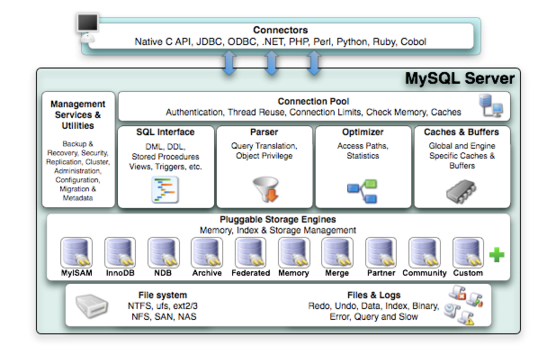
\includegraphics[width=17cm,height= 10cm]{arch}
				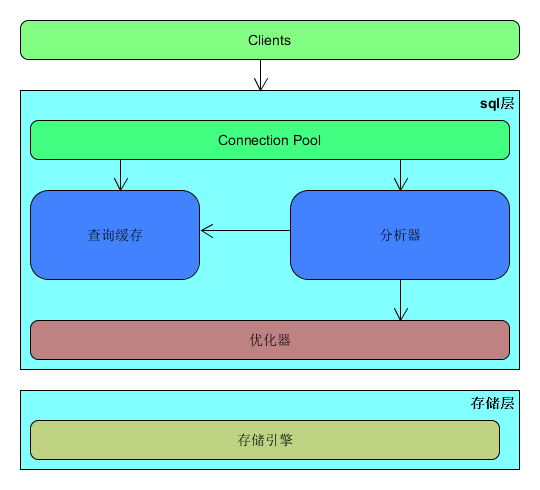
\includegraphics[width=16cm,height= 8cm]{arch2}			
				\caption{mysql 架构}
			\end{figure} 
			
			\verb|Connectors|指的是不同语言中与SQL的交互。
			
			\verb|Management Serveices & Utilities|: 系统管理和控制工具。
			
			\verb|Connection Pool|: 连接池。管理缓冲用户连接,线程处理等需要缓存的需求。
			
			\verb|SQL Interface|: SQL接口。接受用户的SQL命令,并且返回用户需要查询的结果。比如select from就是调用SQL Interface。
			
			\verb|Parser|:解析器。SQL命令传递到解析器的时候会被解析器验证和解析。解析器是由Lex和YACC实现的,是一个很长的脚本。主要功能:
				\begin{itemize}[itemindent = 1em]
					\item 将SQL语句分解成数据结构,并将这个结构传递到后续步骤,以后SQL语句的传递和处理就是基于这个结构的。
					\item 如果在分解构成中遇到错误,那么就说明这个sql语句是不合理的。
				\end{itemize}
			
			\verb|Optimizer|: 查询优化器。
			
			\verb|Cache和Buffer|: 查询缓存。
				\begin{itemize}[itemindent = 1em]
					\item 如果查询缓存有命中的查询结果,查询语句就可以直接去查询缓存中取数据。这个缓存机制是由一系列小缓存组成的。比如表缓存,记录缓存,key缓存,权限缓存等。
				\end{itemize}
			
			\verb|Engine| :存储引擎。
			
			
			\begin{figure}[H]
				\centering
				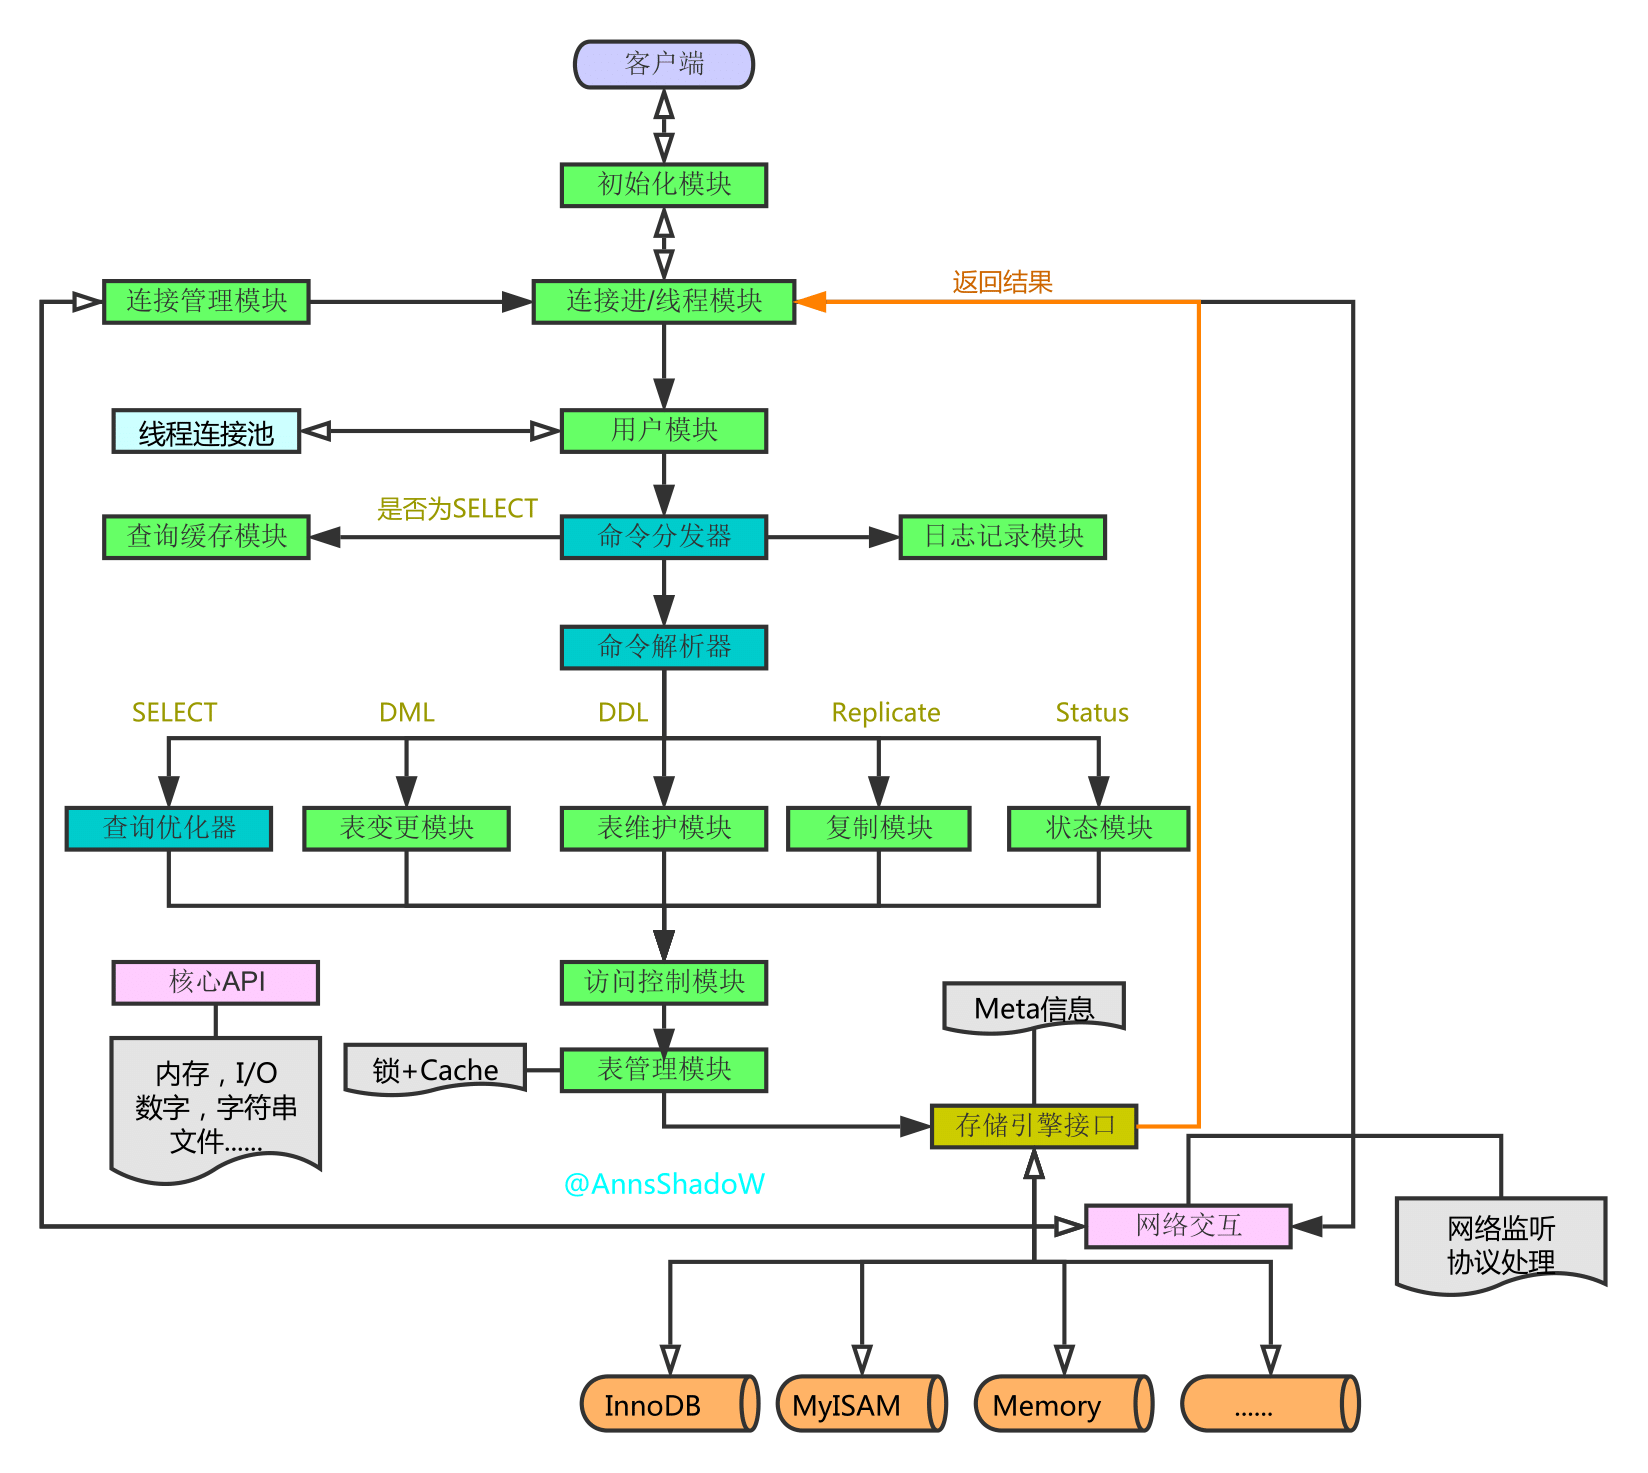
\includegraphics[width=17cm,height= 13cm]{mysqlArch}
				\caption{mysql 架构}
			\end{figure} 			
			
			\verb|mysql|是一个\textbf{C/S架构模型},客户端通过与服务端建立连接来操作服务端数据;
			
			分析器\textbf{分析请求},并转发给优化器;
			
			通过缓存的方式提高查询性能;	
			
			优化器负责和底层的存储引擎进行交互,存储和查询mysql的数据;
		
		\subsection{物理文件组成}
			\begin{itemize}
				\item \textbf{日志文件}:
				\begin{itemize}
					\item \verb|Error log| 错误日志:记录遇到的所有严重的错误信息、每次启动关闭的详细信息;
					\item \verb|Binary log| 二进制日志:也就是binlog,记录所有修改数据库的操作;
					\item \verb|Query log| 查询日志:记录所有查询操作,体积较大,开启后对性能有影响;
					\item \verb|Slow Query log| 慢查询日志:记录所有执行时间超过\verb|long_query_time|的sql语句和达到\verb|min_examined_row_limit|条距离的语句;
					\item \verb|InnoDB redo log|:记录InnoDB所做的物理变更和事务信息;
				\end{itemize}
				
				\item \textbf{数据文件}:
				\begin{itemize}
					\item \verb|.frm文件|:表结构定义信息
					\item \verb|.MYD文件|:MyISAM引擎的数据文件;
					\item \verb|.MYI文件|:MyISAM引擎的索引文件;
					\item \verb|.ibd文件|和\verb|.ibdata文件|:\textbf{InnoDB的数据和索引};\verb|.ibdata|配置为共享表空间时使用,\verb|.ibd|配置为独享表空间时使用;
				\end{itemize}
				
				\item \textbf{其他文件}:
				\begin{itemize}
					\item \verb|系统配置文件|:\verb|/etc/my.cnf|
					\item \verb|pid文件|:存储自己的进程ID
					\item \verb|Unix Socket文件|:连接客户端使用
				\end{itemize}
			\end{itemize}
		
				
	 \section{教程集合地址}
	 	\url{https://blog.csdn.net/orangleliu/article/details/54694272}
	 	
	 	DB入门笔记:\url{https://www.cnblogs.com/ggjucheng/archive/2012/11/02/2751119.html}
	 	
\chapter{数据库基本操作}
	\section{SQL 分类}
		\begin{itemize}
			\item 数据库查询:代表关键字 \verb|select|
			\item 数据库操纵:代表关键字 \verb|insert delete update|
			\item 数据库定义:代表关键字 \verb|create drop alter|
			\item 事务控制:代表关键字 \verb|commit rollback|
			\item 权限控制:代表关键字 \verb|grant revoke|
		\end{itemize} 
	
	\section{常用命令}
		\begin{table}[H]
			\centering
			\caption{常用命令}
			\begin{tabular}{p{4cm}<{\centering}|p{11cm}<{\centering}}
				\hline
					类型  & 命令 \\
				\hline
					显示当前的数据库们  & \verb|show databases;| \\
					使用某个数据库	& 	\verb|use databaseName;| \\
					显示数据库中的表们	& \verb|show tables;|	\\
					查看表的创建语句	& \verb|show create table tableName;|	\\
					查看表的结构	& \verb|desc tableName;|	\\
					重名命(列名、表明)	& \verb|as| ,如 \verb|select lower(ename) as E from emp;|	\\
					创建数据库	& \verb|create database Name;|	\\
					设置字符集	& \verb|set NAMES 'utf8';| \verb|SET character_set_xx = utf8;|	\\
					终止一条语句	& \verb|\c|	\\
				\hline
			\end{tabular}
		\end{table}

	\section{MySql 查询执行流程}
		\url{https://www.cnblogs.com/annsshadow/p/5037667.html}
			
		\subsection{连接}
			\begin{enumerate}
				\item 客户端\textbf{发起一条Query请求},监听客户端的‘连接管理模块’接收请求
				\item 将请求\textbf{转发到}‘连接进/线程模块’
				\item 调用‘用户模块’来进行\textbf{授权}检查
				\item 通过检查后,‘连接进/线程模块’\textbf{从‘线程连接池’中取出空闲的被缓存的连接线程和客户端请求对接},如果失败则创建一个新的连接请求
			\end{enumerate}
		
		\subsection{处理}
			\begin{enumerate}
				\item \textbf{先查询缓存},检查Query语句是否完全匹配,接着再检查是否具有权限,\textbf{都成功则直接取数据返回}
				\item 上一步有失败则转交给‘命令解析器’,经过\textbf{词法分析,语法分析}后生成解析树
				\item 接下来是预处理阶段,处理解析器无法解决的语义,\textbf{检查权限}等,生成新的解析树
				\item 再转交给对应的模块处理
				\item 如果是\verb|SELECT|查询还会经由‘\textbf{查询优化器}’\textbf{做大量的优化},\textbf{生成执行计划}
				\item 模块收到请求后,通过‘访问控制模块’检查所连接的用户是否有访问目标表和目标字段的权限
				\item 有则调用‘表管理模块’,先是查看table cache中是否存在,有则直接对应的表和获取锁,否则重新打开表文件
				\item 根据表的\textbf{meta数据},获取表的存储引擎类型等信息,通过接口调用对应的存储引擎处理
				\item 上述过程中产生数据变化的时候,\textit{若打开日志功能},则会记录到相应\textbf{二进制日志文件}中
			\end{enumerate}
		
		\subsection{结果}
			\begin{enumerate}
				\item Query请求完成后,将结果集返回给‘连接进/线程模块’
				\item 返回的也可以是相应的状态标识,如成功或失败等
				\item ‘连接进/线程模块’进行后续的清理工作,并继续等待请求或断开与客户端的连接
			\end{enumerate}
			
			\begin{figure}[H]
				\centering
				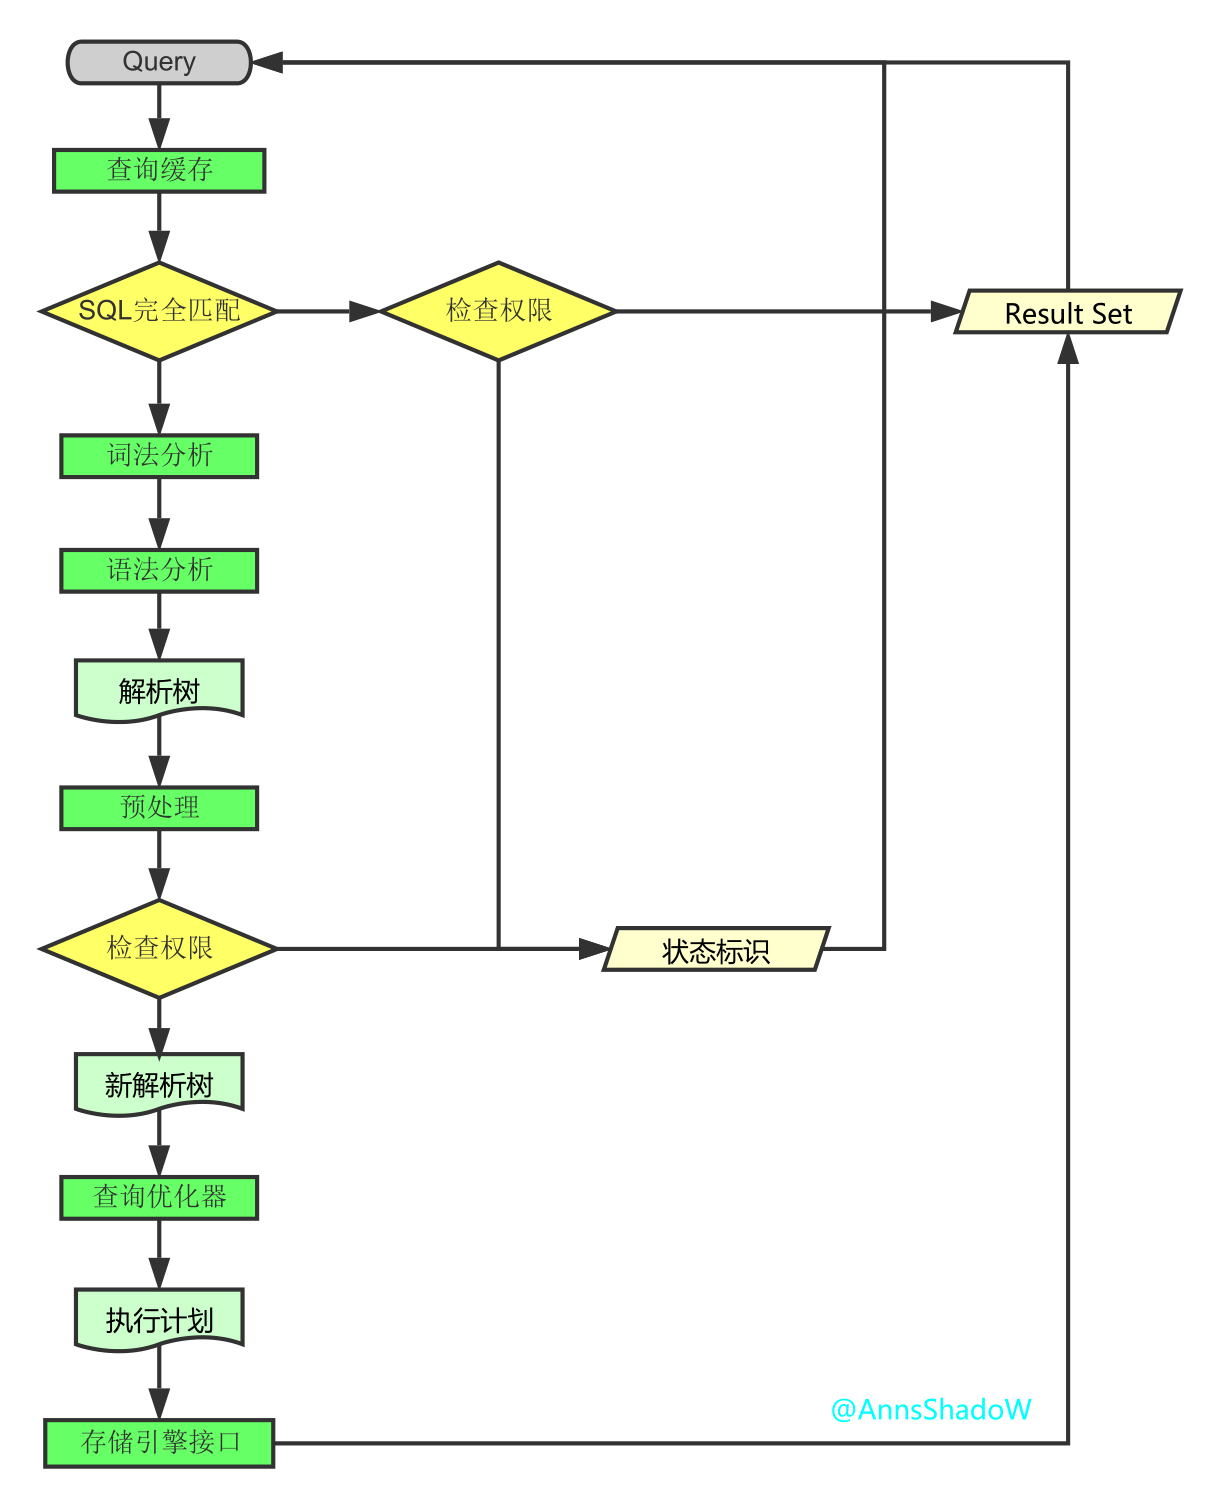
\includegraphics[width=17cm,height=13cm]{mysqlProcess}
				\caption{查询执行流程}
			\end{figure}
			
\chapter{查询}
	\section{基本查询语句}
		\subsection{条件查询}
				\begin{table}[H]
					\centering
					\caption{查询符号}
					\begin{longtable}{c|m{10cm}}
						\hline
						运算符   &   功能说明\\
						\hline
						\verb|=| &  等于 \\
						\verb|!=| & 不等于 \\
						\verb|between ... and ..| & 等同于 \verb|>= ... and <= ...| \\
						\verb|is null| & 为\verb|null(is not null 不为空)| \\
						\verb|and| & 并且 \\
						\verb|or| & 或者\\
						\verb|in| & 包含,相当于多个\verb|or|,(not in 不在这个范围内)\\
						\verb|not| & 取非\\
						\verb|like| & 为模糊查询,支持\verb|%|或\verb|_|匹配,其中\verb|%|匹配任意个字符,\verb|_|只匹配一个字符\\
						\hline	
					\end{longtable}
				\end{table}
				
		\verb|example ->| 
			\begin{lstlisting}
// 执行顺序
	select  // 3
		xx, xx2, xx3
	 from   // 1
		XX
	 where  // 2
		 xx = xx;
		 
// in 示例	查找job是什么的,不是什么的	 
	select 
		ename,job
	from
		emp
	where
		job in('MANAGER','SALESMAN');
		
	select 
		ename,job
	from
		emp
	where
		job not in('MANAGER','SALESMAN');

// like 示例, 查找以S 开头的名字
	select 
		ename
	from 
		emp
	where
		ename like 'S%'	
			\end{lstlisting}
			
		\subsection{排序}
			\verb|order  by|
		
			\begin{lstlisting}
// order  示例 默认升序,(desc 降序)
select 
	ename,salary
from
	emp
order by
	salary

// 按照第几个字段排序	
select 
	ename,salary // 1,2 字段
from
	emp
order by
	2  // 第2个字段
	
// 多个字段排序, ename 升序,salary 降序,使用逗号分割
select 
	ename,salary
from
	emp
order by
	salary desc, ename
			\end{lstlisting}
		
		
		\subsection{数据处理函数(单行)}处理单行后结束
			\begin{itemize}[itemindent = 2em]
				\item \verb|lower| :转换小写
				\item \verb|upper| :转换大写
				\item \verb|substr| :取子串(被截取的串,起始位置,截取长度)
				\item \verb|length| :取长度
				\item \verb|trim| :去空格
				\item \verb|round| :四舍五入
				\item \verb|rand()| :生成随机数
				\item \verb|ifnull(xx, num)|: 可以将\verb|null| 值转换成一个具体值
			\end{itemize}
		
		
		\subsection{分组函数、聚合函数(多行)}
		
			处理多行后结束,自动忽略空值
			
			\textbf{先分组,然后再执行分组函数}, 而where在分组函数之前执行,所以不能
			
			\verb|where| 中不能出现分组函数
			
			\begin{itemize}[itemindent = 2em]
				\item \verb|count |:取得记录数
				\item \verb|sum |:求和
				\item \verb|avg |:求平均
				\item \verb|max |:取最大值
				\item \verb|min |:取最小值
			\end{itemize}
			
			\verb|distinct 去重关键字 -> select distinct job from emp;|  只能出现在所有\textbf{字段}的最前面
			
			\verb|select count(distinct job) from emp;|
			
	\section{分组查询}
			\subparagraph{group by}: \textbf{通过哪个或哪些字段进行分组},使用后select 后只能跟参与分组的字段和分组函数。
			
				\verb|example->| 找出每个工作岗位的最高薪水【先按照工作岗位分组,使用max 函数求每一组的最高工资】
				
					\begin{lstlisting}
// 先按照job 分组,然后对每一组使用max(salary) 求最大值。					
	select 			//3
		max(salary)
	from			//2
		emp;
	group by		//1
		job;	
		
// 结合where 限定分组前条件,即分组前过滤
	select
		job, max(sal)
	from 
		emp
	where 
		job != 'MANAGER'
	group by
		job;
	
					\end{lstlisting}
			
				\verb|example->| 找出每个工作岗位的平均薪水,要求显示平均薪水大于1500
				 where  处理不了
				
			\subparagraph{having} 与where 都是为了完成数据的过滤, \verb|where| 和 \verb|having| 后面都是添加过滤条件,\textbf{where是 在group by 之前执行}, \textbf{而having 是在group  by  后执行}。
			
				\begin{lstlisting}
//上例子解法
select 
	job,avg(sal)
from 
	emp
group by
	job
having 
	avg(sal) >  1500;
 
				\end{lstlisting}
			
			
			\subsection{查询语句总结}
			
				\subparagraph{关键字顺序不能变}:
				
					\begin{lstlisting}
	select 
		...
	from
		...
	where
		...
	group by
		...
	having
		...
	order by
		...
					\end{lstlisting}
			
				\subparagraph{执行顺序}:
					\begin{enumerate}[itemindent = 2em]
						\item \verb|from| 从某张表中检索数据
						\item \verb|where| 经过某条件进行过滤
						\item \verb|group by| 然后分组
						\item \verb|having| 分组之后不满意再过滤
						\item \verb|select| 查询出来
						\item \verb|order by| 排序输出
					\end{enumerate}
		
\section{连接查询}
	查询的时候\textbf{只从一张表检索数据}称为单表查询
	
	在实际的开发中,数据并不是存储在一张表中的,是同时存储在多张表中,这些表和表之间存在关系,我们在检索的时候通常需要将多长表联合起来取得有效数据,这种\textbf{多表查询}被\textbf{称为连接查询}或者叫做跨表查询。
	
	连接查询根据连接方式可以分为如下方式:
		\begin{itemize}[itemindent = 2em]
			\item  内连接
				\begin{itemize}[itemindent = 3em]
					\item 等值连接
					\item 非等值连接
					\item 自连接
				\end{itemize}
				
			\item  外连接
				\begin{itemize}[itemindent = 3em]
					\item 左外连接
					\item 右外连接
				\end{itemize}
				
			\item  全连接【几乎不用】
		\end{itemize}
		
		\begin{figure}[H]
			\centering
			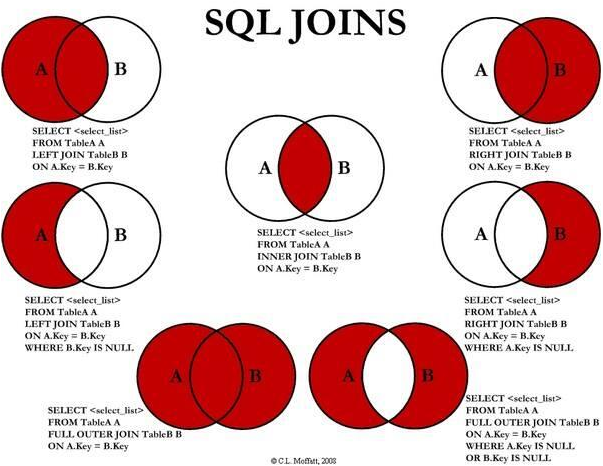
\includegraphics[scale=.76]{joins}
			\caption{SQL Joins}
		\end{figure}
		
	\subsection{内连接}		
			查找两张表匹配的数据。
			
			A表和B表能够完全匹配的记录查询出来,被称为内连接。
			\begin{figure}[H]
				\centering
				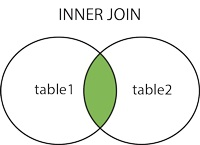
\includegraphics[scale=1]{innoJoin}
				\caption{内连接}
			\end{figure}
			
			\subparagraph{别名的使用,内连接的等值连接} 在进行多表连接查询的时候,尽量给表起别名,这样效率高,可读性高
				\begin{lstlisting}
// 将表emp 用别名 e表示..	

// 查询员工名与其对应的部门名
	select	
		e.ename, d.dname
	from 
		emp e, dept d;
	where 
		e.depno = d.depno
		
// SQL99 语法,使得表连接独立出来了,结构更清晰
	select 
		e.ename, d.dname
	from 
		emp e
	join	  // 内连接的inner 可以省略 
	    dept d
	on 
		e.depno = d.depno;
					\end{lstlisting}
					
				\subparagraph{内连接的非等值连接} 范围
					\begin{lstlisting}
// 找出员工名, 薪水,与其的薪水等级
	select 	
		e.name, e.sal, s.grade
	from
		emp e
	join 
		salgrade s
	on e.sal >= s.lower and e.sal <= s.higher;  // 可以使用between and 替代
					\end{lstlisting}
				 
				
				\subparagraph{内连接的自连接} 自己与自己连接,将自己视为两张表
					\begin{lstlisting}
//  找出每一个员工的上级领导,要求显示员工名以及对应的领导名
	表结构:
	empno ename mgr
	7369  SMITH 7123

// 要点:将自己视为两张表
	select
		a.ename empname, b.ename leaderName
	from 
		emp a
	join
		emp b
	on 
		a.mgr = b.empno;
					\end{lstlisting}	
				
	\subsection{外连接}

		A表和B表能够匹配的记录查询出来之外,\textbf{将其中一张表的记录}\textit{\underline{完全无条件}}的\textbf{完全查询出来},\textit{对方表没有匹配的记录,会自动模拟出NULL与之匹配}。
		
		$$\verb|外连接查询的结构条数| >= \verb|内连接的查询结果数量|$$
		
		可以添加除了内连接外的其他数据。
		\begin{figure}[H]
			\centering
			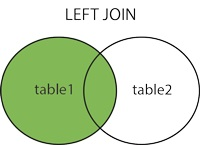
\includegraphics[scale=1]{leftjoin}
			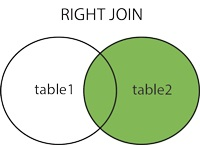
\includegraphics[scale=1]{rightjoin}
			\caption{外连接(左右)}
		\end{figure}
		
		
		\verb|example ->|找出每一个员工对应的部门名称,并且显示所有部门名称,注意部门可能没有员工。
		
				
		\subparagraph{左外连接}
			\verb|select e.ename, d.dname  from dept d left join emp e on e.deptno = d.deptno;|
		
		\subparagraph{右外连接}
			\verb|select e.ename, d.dname  from emp e right join dept d on e.deptno = d.deptno;|// outer  省略
				
		
		\subparagraph{总结}
			\textbf{希望将哪边表的数据完全显示出来},\verb| join| 的前边的修饰词 \verb|right left| 可以恰好说明,如上,\textbf{希望将dept表完全显示},那么\verb|先写dept| 的话,那么就在\verb|join 的左边|,就是 \verb|left join|.	
			
	
	\subsection{内连接外连接 原理性能分析}
		\url{https://www.cnblogs.com/cdf-opensource-007/p/6507678.html}
		
		\url{https://www.cnblogs.com/cdf-opensource-007/p/6517627.html}
	
	\section{子查询}
		\url{https://www.cnblogs.com/zhuiluoyu/p/5822481.html}
	
	\section{union}
		UNION 操作符用于合并两个或多个 SELECT 语句的结果集
		
		\begin{lstlisting}
	SELECT column_name(s) FROM table_name1 // 如只有 1
	UNION
	SELECT column_name(s) FROM table_name2 // 如只有 2
	
	// 则结果为
	1
	2
		\end{lstlisting}	
		
		示例:\url{http://www.w3school.com.cn/sql/sql_union.asp}
			
	\section{limit}		
		用来获取一张表中的\textbf{某部分数据},只在MySQL数据特有的。
		\begin{lstlisting}
	// 找到员工表中前5条记录
	select ename 
	from emp 
	limit 5; //从下标0开始
	
	select ename
	from emp
	limit 0,5;// 从0下标开始,查找前5条
	
	// 找到工资在3到9名的员工
	select salary 
	form emp
	order by salary desc 
	limit 2,7;// 第三个的下标为2,一共7条
		\end{lstlisting}
	
	
	\section{执行顺序}
		\begin{figure}[H]
			\centering
			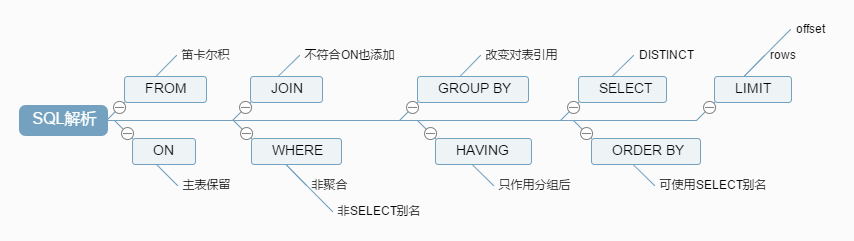
\includegraphics[scale=.6]{sqlProcess}
			\caption{SQL 解析顺序}
		\end{figure}
		
		\begin{lstlisting}
	FROM <left_table>
	ON <join_condition>
	<join_type> JOIN <right_table>
	WHERE <where_condition>
	GROUP BY <group_by_list>
	HAVING <having_condition>
	SELECT 
	DISTINCT <select_list>
	ORDER BY <order_by_condition>
	LIMIT <limit_number>
		\end{lstlisting}
		
	\section{执行过程}
		\url{https://www.cnblogs.com/cdf-opensource-007/p/6502556.html}
		
		\begin{enumerate}
			\item \textbf{加载数据表至内存}:一条查询的sql语句\textbf{先执行的是} \verb|FROM student| 负责\textbf{把数据库的表文件加载到内存中去}。(mysql数据库在计算机上也是一个进程,cpu会给该进程分配一块内存空间)
			\item \textbf{条件过滤}:\verb|WHERE grade < 60|,会把所示\textit{表中的数据进行过滤},\textbf{取出符合条件的记录行,生成一张临时表}
			\item \textbf{分组}:\verb|GROUP BY `name`|会把临时表在内存中切分成若干临时表。
			\item \textbf{选择}:\textbf{SELECT 的执行读取规则}分为sql语句中有无GROUP BY两种情况。
				\begin{itemize}
					\item 当没有GROUP BY时,SELECT 会根据后面的字段名称对内存中的一张临时表整列读取。
					\item 当查询sql中有GROUP BY时,会对内存中的若干临时表分别执行SELECT,而且只取各临时表中的第一条记录,然后再形成新的临时表。这就决定了查询sql使用GROUP BY的场景下,SELECT后面跟的一般是参与分组的字段和聚合函数,否则查询出的数据要是情况而定。另外聚合函数中的字段可以是表中的任意字段,需要注意的是聚合函数会自动忽略空值。
				\end{itemize}
			\item \textbf{对分组后的数据再次过滤}:\verb|HAVING num >= 2|对上图所示临时表中的数据再次过滤,与\verb|WHERE语句|不同的是\verb|HAVING| 用在\verb|GROUP BY|之后,\verb|WHERE|是对\verb|FROM student|从数据库表文件加载到内存中的原生数据过滤,而\verb|HAVING |是对\verb|SELECT |语句执行之后的临时表中的数据过滤。
			\item \textbf{对以上的临时表进行排序}:\verb@ORDER BY xx DESC|ASC@
		\end{enumerate}
		
	
	
	\section{视图 View}
		一种虚拟的表,将查询封装到该视图中。
		
		视图可以包含表的全部或者部分记录,也可以由一个表或者多个表来创建。使用视图就可以不用看到数据表中的所有数据,而是只想得到所需的数据。当我们创建一个视图的时候,\textbf{实际上是}\textit{在数据库里执行了}\verb|SELECT|\textit{语句},\verb|SELECT|\textit{语句包含了字段名称、函数、运算符,来给用户显示数据}。
		
		视图在外观上和表很相似,但是它不需要实际上的物理存储,\textbf{数据还是存储在原来的表里}。\textit{在数据库中,只存放了视图的定义}。
		
		视图的\textbf{使用方式与表的使用方式一致}。
		
		基于视图可以创建视图。
		
		视图\textbf{增加了数据的安全性和逻辑独立性},数据库的设计和结构不会受到视图中的函数、where 或 join 语句的影响。视图可以只展现数据表的一部分数据,对于我们不希望让用户看到全部数据,只希望用户看到部分数据的时候,可以选择使用视图。
		
		更新视图可以更新真实表。
		
		\subsection{创建}
			\begin{lstlisting}
	CREATE [ALGORITHM = {MERGE  | TEMPTABLE | UNDEFINED}]  VIEW 视图名称[(column_list)] AS SELECT 语句  WITH  [CASCADED|LOCAL] CHECK OPTION
	
	create view employee_view as SELECT * from employee;			
			\end{lstlisting}
			首先,第一个中括号里代表的就是创建视图是的算法属性,它允许我们控制\verb|mysql|在创建视图时使用的机制,并且\verb|mysql|提供了三种算法:\verb|MERGE|,\verb|TEMPTABLE| 和 \verb|UNDEFINED|。	
			
			
			\begin{itemize}
				\item \textbf{使用MERGE算法},mysql首先\textbf{将输入查询与定义视图的select语句组合成单个查询。 然后mysql执行组合查询返回结果集}。 \textit{如果}select语句\textbf{包含集合函数}(如min,max,sum,count,avg等)\textbf{或}distinct,group by,havaing,limit,union,union all,\textbf{子查询},\textbf{则不允许使用MERGE算法}。 \textit{如果}select\textbf{语句无引用表},\textbf{则也不允许使用MERGE算法}。 如果不允许MERGE算法,mysql将算法更改为UNDEFINED。我们要注意,将视图定义中的输入查询和查询组合成一个查询称为视图分辨率。
				
				\item \textbf{使用TEMPTABLE算法},mysql首先\textbf{根据定义视图的SELECT语句创建一个临时表,然后针对该临时表执行输入查询}。因为mysql必须创建临时表来存储结果集并将数据从基表移动到临时表,所以TEMPTABLE算法的效率比MERGE算法效率低。 另外,\textbf{使用TEMPTABLE算法的视图是不可更新的}。
				
				\item \textit{当我们创建视图而不指定显式算法时},\textbf{UNDEFINED是默认算法}。 UNDEFINED算法使mysql可以选择使用MERGE或TEMPTABLE算法。mysql优先使用MERGE算法,因为MERGE算法效率更高。
			\end{itemize}
			
			\begin{itemize}
				\item \verb|CASCADED| 默认值,表示更新视图的时候,要满足视图和表的相关条件
				\item \verb|LOCAL|:表示更新视图的时候,要满足该视图定义的一个条件即可
			\end{itemize}
			
			\verb|with check option|:对视图进行更新操作的时,需要检查更新后的值是否还是满足视图公式定义的条件。通俗点,就是所更新的结果是否还会在视图中存在。如果更新后的值不在视图范围内,就不允许更新如果创建视图的时候,没有加上\verb|with check option|,更新视图中的某项数据的话,mysql并不会进行有效性检查。删掉了就删掉了。在视图中将看不到了。所以使用WHIT [CASCADED|LOCAL] CHECK OPTION选项可以保证数据的安全性
			
		\subsection{查看视图数据}
			\begin{lstlisting}
	SELECT * FROM employee_view;		
			\end{lstlisting}		
		
		\subsection{查看视图}	
			\begin{lstlisting}
	show CREATE view employee_view;		
			\end{lstlisting}		
		
		\subsection{删除视图}
			\begin{lstlisting}
	drop view employee_view		
			\end{lstlisting}		
		
		\subsection{修改视图}
			\begin{lstlisting}
	create or replace view employee_view as select eid,ename,salary FROM employee;
	
	alter view employee_view as SELECT * FROM employee;		
			\end{lstlisting}		
		
		\subsection{修改视图中的数据}
			\begin{lstlisting}
	UPDATE employee_view set ename='小红' WHERE ename='小个';		
			\end{lstlisting}	
		
\chapter{增、删、改}
	\section{表、(with约束)}
		\subsection{create table tableName(columName type(length) [constraints]);}
			\begin{lstlisting}
	create table tableName(
		columnName dataType(length) constraints,
		...
	);
	set character_set_result = 'gbk';
	
	drop table tableName;
	drop table if exist tableName; //MySql 特色
	
	create table tableName as select * from existTableName; // 根据已创建的表创建新表
			\end{lstlisting}
		
		\subsection{数据类型}
			\begin{itemize}
				\item \verb|VARCHAR |可变长度字符串
				\item \verb|CHAR |定长字符串
				\item \verb|INT、BIGINT、FLOAT、DOUBLE | 基础数据类型
				\item \verb|DATE | 日期类型
				\item \verb|BLOB | 2进制大对象->图片
				\item \verb|CLOB | 字符大对象->比较大的字符串
			\end{itemize}
			
	\section{表结构}	
		\subsection{alter table tableName add newColumeName type(length);}
		
		\subsection{alter table tableName modify column newType(lenght);}
		
		\subsection{alter table tableName drop column;}
	
	
		
	\section{数据}
		\subsection{insert into tableName(column,..) values (value1,...);}
		
		\subsection{update tableName set columnName=newValue,... where xx;}
			当不指定条件时,将全表的该字段全部更新。
		
		\subsection{delete from tableName where xx;}
	
	
		
	\section{约束}
		\subsection{非空约束 not null}
			不能为空
			
		\subsection{唯一性约束 unique}
			不能重复但是可以为NULL,该字段值具有唯一性
			
			\paragraph{列级约束}
				\begin{lstlisting}
	create table tb(
	..,
	column varchar(32) unique,
	..);
				\end{lstlisting}
				
			\paragraph{表级约束}
				\begin{lstlisting}
	create table tb(
		...,
		column varchar(32),
		...,
		constraint consName unique(column1,...)
	);
				\end{lstlisting}
			
			当使用表级约束时,表示\textbf{多个字段联合}起来后唯一即可。而表级约束可以有名称是为了以后方便删除该约束。
			
		\subsection{主键约束 primary key}
			此列必须是\textbf{唯一并且非空}
			
			每个表都应该有一个主键,并且每个表只能有一个主键。但是注意,并不是说该主键只能在一列上作用,它具有表级约束的联合约束特性。
			\begin{lstlisting}
CREATE TABLE Persons
(
	P_Id int NOT NULL,
	LastName varchar(255) NOT NULL,
	FirstName varchar(255),
	Address varchar(255),
	City varchar(255),
	CONSTRAINT pk_PersonID PRIMARY KEY (P_Id,LastName)
)

			\end{lstlisting}
			在上面的实例中,只有一个主键 \verb|PRIMARY KEY(pk_PersonID),|然而,\verb|pk_PersonID| 的值是由两个列\verb|P_Id 和 LastName)|组成的。
			
		\subsection{外键约束 foreign key}
			\textbf{一个表中的} \verb|FOREIGN KEY| \textbf{指向另一个表中的} \verb|PRIMARY KEY|.
			
			\textbf{“Persons” 表}中的 \verb|“P_Id”| 列\textbf{是 “Persons” 表}中的 \verb|PRIMARY KEY|。
			
			\textbf{“Orders” 表}中的 \verb|“P_Id” |列\textbf{是 “Orders” 表}中的 \verb|FOREIGN KEY|。
			
			\verb|FOREIGN KEY| 约束用于\textbf{预防破坏表之间连接的行为}。
			
			\verb|FOREIGN KEY| 约束也能\textbf{防止非法数据插入外键列},\textit{因为它必须是它指向的那个表中的值之一}。
			
			\begin{lstlisting}
CREATE TABLE Orders
(
	O_Id int NOT NULL,
	OrderNo int NOT NULL,
	P_Id int,
	PRIMARY KEY (O_Id),
	FOREIGN KEY (P_Id) REFERENCES Persons(P_Id)
)
			\end{lstlisting}
	
	
	
	\section{触发器 Trigger}
		触发器\textbf{是与表有关的数据库对象},在满足定义条件时触发,并执行触发器中定义的语句集合。触发器的这种特性可以协助应用在数据库端确保数据的完整性。
	
		\begin{figure}[H]
			\centering
			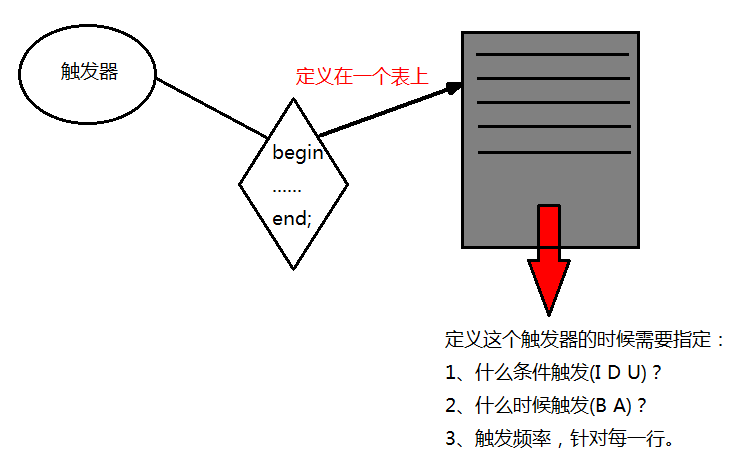
\includegraphics[width=15cm,height=5cm]{trigger}
			\caption{触发器结构演示}
		\end{figure}
		
		\subparagraph{特性}
			\begin{itemize}
				\item 有\verb|begin end|体,\verb|begin end|;之间的语句可以写的简单或者复杂
				\item \textbf{什么条件}会触发:Insert、Update、Delete
				\item \textbf{什么时候}触发:在增删改\textbf{前或者}后
				\item 触发频率:\textbf{针对每一行执行}
				\item 触发器定义在表上,附着在表上。
				\item \textbf{cannot} associate a \textbf{Trigger} with a \textbf{TEMPORARY table} or a \textbf{View}.
				\item 触发器是针对每一行的;对增删改非常频繁的表上切记不要使用触发器,因为它会非常消耗资源。 
			\end{itemize}
		
		
		\subsection{创建触发器}
			\begin{lstlisting}
CREATE
    [DEFINER = { user | CURRENT_USER }]
TRIGGER trigger_name
trigger_time trigger_event
ON tbl_name FOR EACH ROW
  [trigger_order]
trigger_body

trigger_time: { BEFORE | AFTER }

trigger_event: { INSERT | UPDATE | DELETE }

trigger_order: { FOLLOWS | PRECEDES } other_trigger_name			
			\end{lstlisting}
		
			 \verb|FOR EACH ROW| 表示任何一条记录上的操作满足触发事件都会触发该触发器,也就是说触发器的\textbf{触发频率是针对每一行数据触发一次}。

			
			\paragraph{创建只有一个执行语句的触发器}
				\begin{lstlisting}
CREATE TRIGGER 触发器名 BEFORE|AFTER 触发事件 ON 表名 FOR EACH ROW 执行语句;				
				\end{lstlisting}
			
			\paragraph{创建有多个执行语句的触发器}
				\begin{lstlisting}
CREATE TRIGGER 触发器名 BEFORE|AFTER 触发事件
ON 表名 FOR EACH ROW
BEGIN
        执行语句列表
END;				
				\end{lstlisting}
		
		
		\subsection{查看触发器}	
			\begin{itemize}
				\item \verb|SHOW TRIGGERS;|
				\item \verb|SELECT * FROM information_schema.triggers;|
			\end{itemize}
			
			
		\subsection{删除触发器}
			\begin{lstlisting}
DROP TRIGGER [IF EXISTS] [schema_name.]trigger_name
			\end{lstlisting}


\chapter{存储过程}
	\url{http://www.runoob.com/w3cnote/mysql-stored-procedure.html}
	
	存储过程就\textbf{类似于脚本}。
	
	存储过程是\textbf{为了完成特定功能的SQL语句集},经编译创建并保存在数据库中,用户可通过指定存储过程的名字并给定参数(需要时)来调用执行。
	
	\section{存储过程的创建和调用}
		\begin{lstlisting}
CREATE
    [DEFINER = { user | CURRENT_USER }]
 PROCEDURE sp_name ([proc_parameter[,...]])
    [characteristic ...] routine_body
 
proc_parameter:
    [ IN | OUT | INOUT ] param_name type
 
characteristic:
    COMMENT 'string'
  | LANGUAGE SQL
  | [NOT] DETERMINISTIC
  | { CONTAINS SQL | NO SQL | READS SQL DATA | MODIFIES SQL DATA }
  | SQL SECURITY { DEFINER | INVOKER }
 
routine_body:
  Valid SQL routine statement
 
[begin_label:] BEGIN
  [statement_list]
    ……
END [end_label]		
		\end{lstlisting}
	
	
		\subsection{声明语句结束符}
			\begin{lstlisting}
DELIMITER $$
或
DELIMITER //			
			\end{lstlisting}
		
		\subsection{声明存储过程}
			\begin{lstlisting}
CREATE PROCEDURE demo_in_parameter(IN p_in int)       			
			\end{lstlisting}		
		
		\subsection{存储过程开始和结束符号}
			\begin{lstlisting}
BEGIN .... END  			
			\end{lstlisting}
		
		\subsection{变量赋值}
			\begin{lstlisting}
SET @p_in=1  			
			\end{lstlisting}
		
		\subsection{变量定义}		
			\begin{lstlisting}
DECLARE l_int int unsigned default 4000000; 			
			\end{lstlisting}
			
		\subsection{创建存储过程、存储函数名(参数)}
			\begin{lstlisting}
create procedure 存储过程名(参数)			
			\end{lstlisting}		
		
		\subsection{存储过程体}
			\begin{lstlisting}
create function 存储函数名(参数)			
			\end{lstlisting}			
		
		\subsection{实例}
			\begin{lstlisting}
mysql> delimiter $$  #将语句的结束符号从分号;临时改为两个$$(可以是自定义)
mysql> CREATE PROCEDURE delete_matches(IN p_playerno INTEGER)
    -> BEGIN
    ->   DELETE FROM MATCHES
    ->    WHERE playerno = p_playerno;
    -> END$$
Query OK, 0 rows affected (0.01 sec)
 
mysql> delimiter;  #将语句的结束符号恢复为分号    			
			\end{lstlisting}
			
			\begin{lstlisting}
mysql> select * from MATCHES;
+---------+--------+----------+-----+------+
| MATCHNO | TEAMNO | PLAYERNO | WON | LOST |
+---------+--------+----------+-----+------+
|       1 |      1 |        6 |   3 |    1 |
|       7 |      1 |       57 |   3 |    0 |
|       8 |      1 |        8 |   0 |    3 |
|       9 |      2 |       27 |   3 |    2 |
|      11 |      2 |      112 |   2 |    3 |
+---------+--------+----------+-----+------+
5 rows in set (0.00 sec)
 
mysql> call delete_matches(57);
Query OK, 1 row affected (0.03 sec)
 
mysql> select * from MATCHES;
+---------+--------+----------+-----+------+
| MATCHNO | TEAMNO | PLAYERNO | WON | LOST |
+---------+--------+----------+-----+------+
|       1 |      1 |        6 |   3 |    1 |
|       8 |      1 |        8 |   0 |    3 |
|       9 |      2 |       27 |   3 |    2 |
|      11 |      2 |      112 |   2 |    3 |
+---------+--------+----------+-----+------+
4 rows in set (0.00 sec)			
			\end{lstlisting}

	\section{存储过程的参数}
	
	
	
	\section{存储过程的变量}


\chapter{游标}
	有数据缓冲的思想:游标的设计\textbf{是一种数据缓冲区的思想,用来存放SQL语句执行的结果}。 
	
	游标是\textit{在先从数据表中检索出数据之后才能继续灵活操作的技术}。 类似于指针:游标类似于指向数据结构堆栈中的指针,用来pop出所指向的数据,并且只能每次取一个。
	
	\section{特点}
		\begin{itemize}
			\item 游标是\textbf{针对行操作的},所以对从数据库中select查询得到的每一行可以进行分开的独立的相同或不同的操作,是一种分离的思想。
			\item 在数据量大的情况下,是不适用的,速度过慢。这里有个比喻就是:当你去ATM存钱是希望一次性存完呢,还是100一张一张的存,这里的100一张一张存就是游标针对行的操作。 数据库大部分是面对集合的,业务会比较复杂,而游标使用\textbf{会有死锁},影响其他的业务操作,不可取。 当数据量大时,使用游标会造成\textbf{内存不足}现象。
		\end{itemize}
	
	\section{创建与使用}
		\subsection{定义游标}
			\begin{lstlisting}
DECLARE <游标名> CURSOR FOR select语句;	

DECLARE mycursor CURSOR FOR select * from shops_info;	
			\end{lstlisting}
		
		\subsection{打开游标}
			\begin{lstlisting}	
open <游标名>			
			\end{lstlisting}
		
		\subsection{使用游标}
			使用游标需要用关键字fetch来取出数据,然后取出的数据需要有存放的地方,我们需要用declare声明变量存放列的数据其语法格式为:
			\begin{lstlisting}
declare 变量1 数据类型(与列值的数据类型相同)
declare 变量2 数据类型(与列值的数据类型相同)
declare 变量3 数据类型(与列值的数据类型相同)
FETCH [NEXT | PRIOR | FIRST | LAST] FROM <游标名> [ INTO 变量名1,变量名2,变量名3[,…] ]			
			\end{lstlisting}
			
			\begin{lstlisting}
-- 声明四个变量
  declare id varchar(20); 
  declare pname varchar(20); 
  declare pprice varchar(20);
  declare pdescription varchar(20);
 
-- 1、定义一个游标mycursor
  declare mycursor cursor for
	select *from shops_info;
-- 2、打开游标
  open mycursor;
-- 3、使用游标获取列数据放入变量中
  fetch  next from mycursor into id,pname,pprice,pdescription; 			
			\end{lstlisting}
			
		\subsection{关闭游标}
			\begin{lstlisting}
close mycursor;			
			\end{lstlisting}
		
		
		\subsection{释放游标}
			\begin{lstlisting}
deallocate mycursor;			
			\end{lstlisting}
		
		
	\section{实例}
		\url{https://www.cnblogs.com/mqxs/p/6018766.html}
		
		\url{https://www.cnblogs.com/progor/p/8875100.html}
		
		\subsection{普通游标}
			\begin{lstlisting}
drop procedure if exists cursor_test;
delimiter //
create procedure cursor_test()
begin
    -- 声明与列的类型相同的四个变量
    declare id varchar(20); 
    declare pname varchar(20); 
    declare pprice varchar(20);
    declare pdescription varchar(20);
 
-- 1、定义一个游标mycursor
    declare mycursor cursor for
   	select *from shops_info;
-- 2、打开游标
    open mycursor;
-- 3、使用游标获取列的值
    fetch  next from mycursor into id,pname,pprice,pdescription; 
-- 4、显示结果
    select id,pname,pprice,pdescription;
-- 5、关闭游标
    close mycursor;
end;
//
delimiter ;
call cursor_test();		
			\end{lstlisting}
		
			当然可以使用循环,while 循环定义如下:
			\begin{lstlisting}
WHILE expression DO
    Statements;
END WHILE
//实例
DECLARE num INT;
DECLARE my_string  VARCHAR(255);
SET num =1;
SET str ='';
  WHILE num  < span>10DO
SET  my_string =CONCAT(my_string,num,',');
SET  num = num +1;
END WHILE;		
			\end{lstlisting}
	
		\subsection{循环游标}	
			\begin{lstlisting}
create procedure p3()
begin
    declare id int;
    declare name varchar(15);
    declare flag int default 0;
    -- 声明游标
    declare mc cursor for select * from class;
    declare continue handler for not found set flag = 1;
    -- 打开游标
    open mc;
    -- 获取结果
    l2:loop 
    
    fetch mc into id,name;
    if flag=1 then -- 当无法fetch会触发handler continue
        leave l2;
    end if;
    -- 这里是为了显示获取结果
    insert into class2 values(id,name);
    -- 关闭游标
    end loop;
    close mc;
    
end;

call p3();-- 不报错
select * from class2;	
			\end{lstlisting}
			
	
\chapter{索引-重要}
	\section{简介}
		索引用于快速找出在某个列中有一特定值的行,不使用索引,MySQL必须从第一条记录开始读完整个表,直到找出相关的行,表越大,查询数据所花费的时间就越多,如果表中查询的列有一个索引,MySQL能够快速到达一个位置去搜索数据文件,而不必查看所有数据,那么将会节省很大一部分时间。

		\textbf{例如}:\textit{有一张person表,其中有2W条记录,记录着2W个人的信息。有一个Phone的字段记录每个人的电话号码,现在想要查询出电话号码为xxxx的人的信息}。
			\begin{itemize}
				\item \textbf{如果没有索引},那么将从表中第一条记录一条条往下\textbf{遍历},直到找到该条信息为止。
				\item \textbf{如果有了索引},那么会将\textbf{该Phone字段},\textbf{通过一定的方法进行存储},\textit{好让查询该字段上的信息时,能够快速找到对应的数据},而不必在遍历2W条数据了。其中MySQL中的索引的存储类型有两种:\verb|BTREE|、\verb|HASH|。
			\end{itemize}

	\section{优点、缺点和使用原则}
		\subparagraph{优点}
			\begin{itemize}[itemindent = 1em]
				\item 所有的MySql\textbf{列类型}(字段类型)\textbf{都可以被索引},也就是\textit{可以给任意字段设置索引}
				\item 大大加快数据的查询速度
			\end{itemize}
			
		\subparagraph{缺点}
			\begin{itemize}[itemindent = 1em]
				\item 创建索引和维护索引要耗费时间,并且随着数据量的增加所耗费的时间也会增加
				\item 索引也需要占空间
				\item 当对表中的数据进行增加、删除、修改时,索引也需要动态的维护,降低了数据的维护速度。
			\end{itemize}
			
		\subparagraph{使用原则}
			通过上面说的优点和缺点,我们应该可以知道,并不是每个字段度设置索引就好,也不是索引越多越好,而是需要自己合理的使用。
			\begin{itemize}[itemindent = 1em]
				\item \textbf{对经常更新的表}就\textit{避免对其进行过多的索引},对经常用于查询的字段应该创建索引
				\item \textbf{数据量小的表最好不要使用索引},因为由于数据较少,可能查询全部数据花费的时间比遍历索引的时间还要短,索引就可能不会产生优化效果
				\item \textbf{在一同值少的列上(字段上)不要建立索引},比如\textit{在学生表的"性别"字段上只有男,女两个不同值}。相反的,在一个字段上不同值较多可是建立索引
			\end{itemize}
			
	\section{索引的分类}
		\subparagraph{存储引擎支持类型}
			索引是在存储引擎中实现的,也就是说不同的存储引擎,会使用不同的索引
			\begin{itemize}[itemindent = 2em]
				\item \verb|MyISAM和InnoDB|存储引擎:\textbf{只支持BTREE索引}
				\item \verb|MEMORY/HEAP|存储引擎:\textbf{支持HASH和BTREE索引}
			\end{itemize}
			
		\subparagraph{单列索引}
			一个索引只包含单个列,但一个表中可以有多个单列索引。主要包括以下几种类型:
			\begin{enumerate}[itemindent = 2em]
				\item 普通索引:基本索引类型,没有什么限制,允许在定义索引的列中插入重复值和空值
				\item 唯一索引:索引列中的值必须是唯一的,但是允许为空值
				\item 主键索引:是一种特殊的唯一索引,不允许有空值。
			\end{enumerate}
			
		\subparagraph{组合索引}
			在表中的多个字段组合上创建的索引,\textbf{只有}在查询条件中\textit{使用了}\textbf{这些字段的左边字段时},索引才会被使用,使用组合索引时遵循最\textbf{左前缀集合}。
		
			\textbf{联合索引左侧字段用了范围查询,则其他字段无法用上}。
			
	\section{创建表添加索引}
		\subparagraph{创建普通索引}
			\begin{lstlisting}
// 方式一
CREATE TABLE book (
bookid INT NOT NULL,               
bookname VARCHAR(255) NOT NULL,           
authors VARCHAR(255) NOT NULL,            
info VARCHAR(255) NULL,                
comment VARCHAR(255) NULL,             
year_publication YEAR NOT NULL,           
INDEX(year_publication)               
);

// 方式二
CREATE TABLE book (
bookid INT NOT NULL,               
bookname VARCHAR(255) NOT NULL,           
authors VARCHAR(255) NOT NULL,            
info VARCHAR(255) NULL,                
comment VARCHAR(255) NULL,             
year_publication YEAR NOT NULL,           
KEY(year_publication)               
);                                                
			\end{lstlisting}
		\subparagraph{创建唯一索引}
			\begin{lstlisting}
CREATE TABLE t1
(
id INT NOT NULL,
name CHAR(30) NOT NULL,
UNIQUE INDEX UniqIdx(id)
); 
			\end{lstlisting}
		\subparagraph{创建主键索引}
			\begin{lstlisting}
CREATE TABLE t2
(
	id INT NOT NULL,
	name CHAR(10),
	PRIMARY KEY(id)
);
			\end{lstlisting}
		
		\subparagraph{创建组合索引}
			\begin{lstlisting}
CREATE TABLE t3
(
	id INT NOT NULL,
	name CHAR(30) NOT NULL,
	age INT NOT NULL,
	info VARCHAR(255),
	INDEX MultiIdx(id,name,age)
);
			\end{lstlisting}
			
			\textbf{组合索引就是遵从了最左前缀},\textit{利用索引中最左边的列集来匹配行,这样的列集称为最左前缀},例如,这里由id、name和age3个字段构成的索引,索引行中就按\verb|id/name/age|的顺序存放,\textbf{索引可以索引下面字段组合}\verb|(id,name,age)|、\verb|(id,name)|或者\verb|(id)|。如果要查询的字段不构成索引最左面的前缀,那么就不会是用索引,比如,age或者\verb|(name,age)|组合\textbf{就不会使用索引查询}
			
	
	\section{在已经存在的表上创建索引}
	
		\verb@ALTER TABLE 表名 ADD[UNIQUE|FULLTEXT|SPATIAL] [INDEX|KEY] [索引名](字段名)[ASC|DESC]@
		
		\verb@CREATE [UNIQUE|FULLTEXT|SPATIAL] [INDEX|KEY] 索引名称 ON 表名(字段名[length])[ASC|DESC]@
		
		\begin{itemize}
			\item ALTER TABLE book ADD INDEX BkNameIdx(bookname(30));
			\item CREATE INDEX BkBookNameIdx ON book(bookname);
		\end{itemize}
	
	\section{删除索引}
		\begin{itemize}
			\item ALTER TABLE 表名 DROP INDEX 索引名;
			\item DROP INDEX 索引名 ON 表名;
		\end{itemize}
	
	\section{索引背后的算法原理}
		\url{http://blog.codinglabs.org/articles/theory-of-mysql-index.html}	
	
	
	\section{索引设计概要}
		\url{https://draveness.me/sql-index-intro}
			
	\section{参考}
		\url{https://www.cnblogs.com/whgk/p/6179612.html}
			
	
	
\chapter{事务}
	\section{概述}
		一般来说,事务是必须满足4个条件(ACID)::原子性(Atomicity,或称不可分割性)、一致性(Consistency)、隔离性(Isolation,又称独立性)、持久性(Durability)。
		
		\begin{itemize}
			\item \textbf{原子性}:\textit{一个事务(transaction)中的所有操作,要么全部完成,要么全部不完成},不会结束在中间某个环节。事务在执行过程中发生错误,会被回滚(Rollback)到事务开始前的状态,就像这个事务从来没有执行过一样。
			\item \textbf{一致性}:在事务开始之前和事务结束以后,数据库的完整性没有被破坏。这表示写入的资料必须完全符合所有的预设规则,这包含资料的精确度、串联性以及后续数据库可以自发性地完成预定的工作。
			\item \textbf{隔离性}:数据库\textit{允许多个并发事务同时对其数据进行读写和修改的能力,隔离性可以防止多个事务并发执行时由于交叉执行而导致数据的不一致}。事务隔离分为不同级别,包括读未提交(Read uncommitted)、读提交(read committed)、可重复读(repeatable read)和串行化(Serializable)。
			\item \textbf{持久性}:事务处理结束后,对数据的修改就是永久的,即便系统故障也不会丢失。
		\end{itemize}
	
	\section{应用}
		用 \verb|BEGIN|, \verb|ROLLBACK|, \verb|COMMIT|来实现.
		
		\verb|BEGIN| \textbf{开始一个事务}
		
		\verb|ROLLBACK| \textbf{事务回滚}
		
		\verb|COMMIT| \textbf{事务确认}
		
		\begin{lstlisting}
mysql> begin;  # 开始事务
Query OK, 0 rows affected (0.00 sec)
 
mysql> insert into runoob_transaction_test value(5);
Query OK, 1 rows affected (0.01 sec)
 
mysql> insert into runoob_transaction_test value(6);
Query OK, 1 rows affected (0.00 sec)
 
mysql> commit; # 提交事务
Query OK, 0 rows affected (0.01 sec)

mysql>  select * from runoob_transaction_test;
+------+
| id   |
+------+
| 5    |
| 6    |
+------+
2 rows in set (0.01 sec)
 
mysql> begin;    # 开始事务
Query OK, 0 rows affected (0.00 sec)
 
mysql>  insert into runoob_transaction_test values(7);
Query OK, 1 rows affected (0.00 sec)
 
mysql> rollback;   # 回滚
Query OK, 0 rows affected (0.00 sec)
 
mysql>   select * from runoob_transaction_test;   # 因为回滚所以数据没有插入
+------+
| id   |
+------+
| 5    |
| 6    |
+------+
2 rows in set (0.01 sec)		
		\end{lstlisting}


\chapter{日志}
	\section{bin-log}
		MySQL的二进制日志可以说是MySQL\textbf{最重要的日志}了,它记录了所有的\textbf{DDL和DML}(除了数据查询语句)语句,\textbf{以事件形式记录,还包含语句所执行的消耗的时间},MySQL的二进制日志是事务安全型的。
		
		二进制有两个最重要的使用场景: 
			\begin{itemize}
				\item 其一:MySQL Replication\textbf{在Master端开启binlog},\textit{Master把它的二进制日志传递给slaves}来达到master-slave数据一致的目的。 
				\item 其二:自然就是数据恢复了,通过使用mysqlbinlog工具来使恢复数据。
			\end{itemize}    
		    
		\subparagraph{参考}
			\url{https://www.cnblogs.com/martinzhang/p/3454358.html}
	
		\subsection{GTID}	
	
	
	
	\section{error-log}
	
	
	\section{slow-query-log}
		MySQL \textbf{慢查询日志}是指 MySQL 中\textbf{执行时间超过} \verb|long_query_time| \textbf{阀值的 SQL 语句}。
		
		\verb|Dumbo| 默认每天零晨 \textbf{rotate 慢查询日志},按日期命名文件,每天一个文件,服务器上保留最近 8 天的慢查询日志文件。
		
		\textit{从慢查询日志中统计出执行比较频繁且执行时间比较久、扫描的行数也比较大的 SQL,可以针对这类 SQL 进行优化。}
	
		\paragraph{参数说明}
			慢查询日志相关的几个参数,有先后依赖关系,顺序如下:
			\begin{enumerate}[itemindent = 2em, itemsep = 0pt,partopsep=0pt]
				\item \verb|slow_query_log| \\ 是否启用慢查询日志功能,慢查询日志的内容可以在 \textbf{Dumbo 管理平台} \textit{实例管理 --> 日志管理 --> 慢查询日志} 上查看
				\item \verb|log_slow_admin_statements| \\ 是否记录administrative statements 语句到慢查询日志里。
				\item \verb|long_query_time| \\ 定义慢查询日志的触发条件,如果 SQL 实际执行时间(不包括锁的时间)超过 \verb|long_query_time| 定义的阀值,此 SQL 则被记录到慢查询日志里。
				\item \verb|min_examined_row_limit| \\ 只有慢查询语句的执行行数检查返回大于该参数指定值,此慢查询语句才被记录到慢查询日志中。
			\end{enumerate}
			
			\begin{table}[H]
				\centering
				\caption{慢查询日志参数}
				\begin{tabular}{p{6cm}<{\centering}|p{3cm}<{\centering}|p{3cm}<{\centering}|p{3cm}<{\centering}}
					\hline
						方法 &  MySQL默认值 &  Dumbo 默认值 & 能否自助修改\\
					\hline
				 \verb|slow_query_log| & OFF & ON &  否 \\
				 \verb|long_query_time| & 10s & 0.1s & 能 \\
				 \verb|log_slow_admin_statements| & OFF & ON & 否 \\
				 \verb|log_slow_slave_statements| & OFF & ON &否\\
				 \verb|min_examined_row_limit| & 0& 100 & 否 \\
					\hline
				\end{tabular}					
			\end{table}
			
			
			因此 \textbf{Dumbo 实例默认配置下},记录慢查询日志的条件是:
			\textbf{SQL 实际执行时间超过 0.1s,且此 SQL 的执行行数检查返回值大于 100}。
		\paragraph{优点}
			\begin{itemize}
				\item 语句调优 \\ 通过统计慢查询日志(可联系 Dumbo 值班),找出最耗时的 top 10 语句,优化完成后,再统计新的慢查询日志,一直重复,直到没有产生新的慢查询语句。
				\item 性能排查 \\ 如果一个实例的 CPU 使用率比较高,可以优先检查一下该实例的慢查询日志,如果慢查询日志刷得比较厉害,可以初步确认是由于 SQL 语句不够优化导致实例 CPU 使用率高,可以通过优化 SQL 来解决。
			\end{itemize}
		
		\paragraph{参考}
			\begin{itemize}
				\item \url{https://www.cnblogs.com/saneri/p/6656161.html}
			\end{itemize}
				


\chapter{存储引擎}
	\section{InnoDB存储引擎}	
	
	
\chapter{集群} 
	\section{备份-重要}
		\begin{itemize}
			\item mysqldump: 逻辑备份; 单线程导入导出; 注意设定字符集; 
			\item mydumper: 逻辑备份; “多线程”导入导出; 无需关心字符集;
			\item innobackup/mysqlbackup: 物理备份; 速度较快;
		\end{itemize}
		\subsection{普通数据库备份}
			\verb|mysqldump -u root -p password --default-character-set=utf-8 dataname > dataname.sql|
			
			\verb|mysql -u root -p password --default-character-set=utf-8 dataname < dataname.sql|
		\subsection{备份到压缩文件}
			\verb@mysqldump -u root -p database | gzip > database.sql.gz@
			
			\verb@gzip < database.sql.gz | mysql -u root -p database@
		\subsection{增量备份}
			\verb@mysqlbinlog bin-log.000002 |mysql -uroot -ppassword@
		

	\section{主从模式-replication}
	
	\section{集群}



\chapter{MySQL 性能优化}
	\begin{figure}[H]
		\centering
		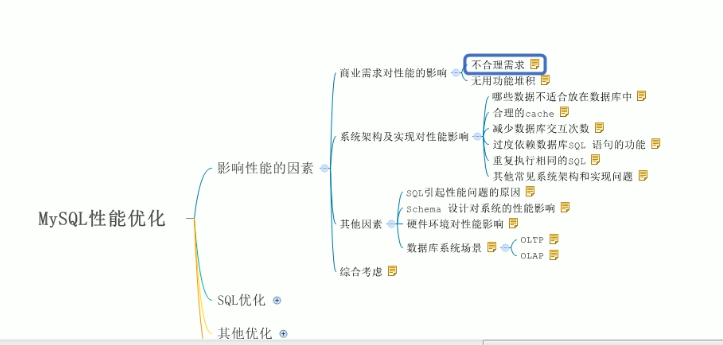
\includegraphics[scale=0.7]{xingNeng}
		\caption{性能优化结构}
	\end{figure}
	
	\section{影响性能的因素}
		\subsection{不合理的需求如何优化}
			需求: 一个论坛帖子总量的统计
			附加要求:实时更新
			
			\begin{itemize}
				\item 初始阶段:\verb|select count(id)|
				\item 新建一个表,在这个表中更新这个汇总数据 (频率问题- update 锁)
				\item 真正的问题在于,实时?创建一个统计表,隔一段时间统计一次并存入(Redis)。
			\end{itemize}
		
		\subsection{无用功能的堆积}
			\begin{itemize}
				\item 无用的列堆积
				\item 错误的表设计
				\item 无用的表关联
			\end{itemize}
		
		
		\subsection{哪些数据不适合放在数据库中}
			\begin{itemize}
				\item 二进制文件-文件-图片
				\item 流水队列数据
				\item 超大文本
			\end{itemize}
		
		
		\subsection{合理的cache}
			哪些数据适合放到cache 中
			\begin{itemize}
				\item 系统的配置信息 
				\item 活跃用户的基本信息 
				\item 活跃用户的定制化信息
				\item 基于时间段的统计信息
				\item 读 >>> 写的数据
			\end{itemize}
		
		\subparagraph{减少数据库交互次数}
		\subparagraph{减少重复执行相同的SQL}
	
		\subsection{其他}
			\begin{itemize}
				\item cache 系统的不合理利用导致Cache 命中率底下造成的数据库访问量的增加,同事也浪费了Cache系统的硬件资源投入
				\item 过度依赖面向对象思想,对系统的可扩展性的过度追求,促使系统设计的时候将对象拆的过于分散,造成系统中大量的复杂join 语句,而MySQL 在各数据库系统中的主要优势在于处理简单逻辑的查询,这与其锁定的机制也有较大关系
				\item 对数据库过度依赖,将大量适合存放于文件系统中的数据存入了数据库中,造成数据库资源的浪费,影响到系统的整体性能,如各种日志信息
				\item 过度理想化系统的用户体验,是大量的非核心业务消耗过多的资源,如大量
			\end{itemize}
			
	\section{Sql 优化}	
	
	\section{Mysql 锁}
		
	\section{MySQL 复制}

	\section{Explain 详解}
		\url{https://www.cnblogs.com/xuanzhi201111/p/4175635.html}
		
		在日常工作中,我们会有时会开慢查询去记录一些执行时间比较久的SQL语句,找出这些SQL语句并不意味着完事了,些时我们常常用到explain这个命令来查看一个这些SQL语句的执行计划,查看该SQL语句有没有使用上了索引,有没有做全表扫描,这都可以通过explain命令来查看。
		
		expain出来的信息有10列,分别是\verb|id|、\verb|select_type|、\verb|table|、\verb|type|、\verb|possible_keys|、\verb|key|、\verb|key_len|、\verb|ref|、\verb|rows|、\verb|Extra|,下面对这些字段出现的可能进行解释:
		
		\subsection{id}
			SQL执行的顺序的标识,SQL从大到小的执行
			\begin{itemize}
				\item id相同时,执行顺序由上至下
				\item 如果是子查询,id的序号会递增,id值越大优先级越高,越先被执行
				\item id如果相同,可以认为是一组,从上往下顺序执行;在所有组中,id值越大,优先级越高,越先执行
			\end{itemize}
			
		\subsection{select\_type}
			\begin{itemize}
				\item \verb|SIMPLE|  :简单SELECT,不使用UNION或子查询等
				\item \verb|PRIMARY| :查询中若包含任何复杂的子部分,最外层的select被标记为PRIMARY
				\item \verb|UNION| :UNION中的第二个或后面的SELECT语句
				\item \verb|DEPENDENT UNION| :UNION中的第二个或后面的SELECT语句,取决于外面的查询
				\item \verb|UNION RESULT| :UNION的结果
				\item \verb|SUBQUERY| :子查询中的第一个SELECT
				\item \verb|DEPENDENT SUBQUERY| :子查询中的第一个SELECT,取决于外面的查询
				\item \verb|DERIVED| :派生表的SELECT, FROM子句的子查询
				\item \verb|UNCACHEABLE SUBQUERY| :一个子查询的结果不能被缓存,必须重新评估外链接的第一行
			\end{itemize}
			
		\subsection{table}	
			显示这一行的数据是关于哪张表的
			
		\subsection{type}
			
			\begin{itemize}
				\item \verb|ALL|:Full Table Scan, MySQL将\textbf{遍历全表}以找到匹配的行
				\item \verb|Index|: Full Index Scan,index与ALL区别为index类型\textbf{只遍历索引树}
				\item \verb|Range|:只检索给定范围的行,使用一个索引来选择行
				\item \verb|Ref|: 表示上述表的连接匹配条件,即哪些列或常量\textbf{被用于查找索引列上的值}
				\item \verb|Eq_ref|: 	类似ref,区别就在使用的索引是唯一索引,对于每个索引键值,表中只有一条记录匹配,简单来说,就是多表连接中使用primary key或者 unique key作为关联条件
				\item \verb|Const|、\verb|System|: 当MySQL对查询某部分进行优化,并转换为一个常量时,使用这些类型访问。如将主键置于where列表中,MySQL就能将该查询转换为一个常量,system是const类型的特例,当查询的表只有一行的情况下,使用system
				\item \verb|NULL|: MySQL在优化过程中分解语句,执行时甚至不用访问表或索引,例如从一个索引列里选取最小值可以通过单独索引查找完成。
			\end{itemize}
			
		\subsection{possible\_keys}
			指出MySQL能使用哪个索引在表中找到记录,查询涉及到的字段上若存在索引,则该索引将被列出,但不一定被查询使用
			
		\subsection{Key}
			key列显示MySQL实际决定使用的键(索引)
			
		\subsection{key\_len}
			表示索引中使用的字节数,可通过该列计算查询中使用的索引的长度(\verb|key_len|显示的值为索引字段的最大可能长度,并非实际使用长度,即\verb|key_len|是根据表定义计算而得,不是通过表内检索出的)
			
			不损失精确性的情况下,长度越短越好 
			
		\subsection{ref}
			表示上述表的连接匹配条件,即哪些列或常量被用于查找索引列上的值
			
		\subsection{rows}
			表示MySQL根据表统计信息及索引选用情况,估算的找到所需的记录所需要读取的行数
	
		\subsection{总结}
			\begin{itemize}
				\item EXPLAIN不会告诉你关于触发器、存储过程的信息或用户自定义函数对查询的影响情况
				\item EXPLAIN不考虑各种Cache
				\item EXPLAIN不能显示MySQL在执行查询时所作的优化工作
				\item 部分统计信息是估算的,并非精确值
				\item EXPALIN只能解释SELECT操作,其他操作要重写为SELECT后查看执行计划。
			\end{itemize}
			

	\section{查询优化-海量数据}
	
	\section{经验Tips}
		\url{https://coolshell.cn/articles/1846.html}
		
		\begin{enumerate}
			\item \textbf{EXPLAIN} \verb|SELECT| 查询 \\ 解释查询语句,查看是否使用到索引(\textbf{Key})
			\item 当只要一行数据时使用 \verb|LIMIT 1|  \\ 这样会在找到一条数据后停止搜索,而不是继续往后查少下一条符合记录的数据
			\item 为搜索字段建索引 \\ BTree Or Hash Better Than All
			\item 在Join表的时候使用相当类型的例,并将其索引
			\item 千万不要 \verb|ORDER BY RAND()|
			\item 避免 \verb|SELECT *|
			\item 永远为每张表设置一个ID
			\item 使用 \verb|ENUM| 而不是 \verb|VARCHAR|
			\item 尽可能的使用 \verb|NOT NULL|
			\item 无缓冲的查询
			\item 把IP地址存成 \verb|UNSIGNED INT|
			\item 固定长度的表会更快
			\item 垂直分割
			\item 拆分大的 DELETE 或 INSERT 语句
			\item 越小的列会越快
			\item 选择正确的存储引擎
		\end{enumerate}
		
\chapter{疑难杂症}
	\section{mysql.sock -ERROR 2002 (HY000)}
		
		\verb|Can't connect to local MySQL server through socket '/tmp/mysql.sock' (2)|
		
		\url{https://blog.csdn.net/hjf161105/article/details/78850658}
		    
\end{document} 
 		    